\documentclass[aspectratio=169,10pt]{beamer}
\usetheme{Madrid}
\usecolortheme{seahorse}
\setbeamertemplate{navigation symbols}{}
\usepackage{amsmath,amssymb}
\usepackage{booktabs}
\usepackage{graphicx}

\newcommand{\mrad}{\,\mathrm{mrad}}

\title[Environment-Limited Synchronization]{Environment-Limited Synchronization:\\
Distributed Arrays That Phase-Lock on Ordinary Traffic}
\author{Chandler Stevenson}
\institute{Princeton University}
\date{\today}

\begin{document}

% ---------------------------------------------------------------- 1
\begin{frame}
  \titlepage
  \begin{center}
    \footnotesize Waveform-level simulation study --- full oscillator and RF impairments; no hardware yet.
  \end{center}
\end{frame}

% ---------------------------------------------------------------- 2
\begin{frame}{The problem: synchronization eats the channel}
  \begin{columns}[T]
    \begin{column}{0.52\textwidth}
      \begin{itemize}
        \item A distributed transmit array only achieves coherent
              beamforming gain while every station's carrier phase is
              locked to the others.
        \item Conventional over-the-air locking uses \emph{dedicated
              two-way exchanges}: stations take turns sending known
              signals; comparing the two directions cancels the
              propagation path and measures the clock offset alone.
        \item That cost is per-station, per-interval. As the array
              grows, synchronization traffic saturates the frame:
              measured collapse at $N\!\approx\!8$ (naive schedule)
              and incoherence by $N\!=\!64$ even for the strongest
              conventional baseline.
      \end{itemize}
    \end{column}
    \begin{column}{0.46\textwidth}
      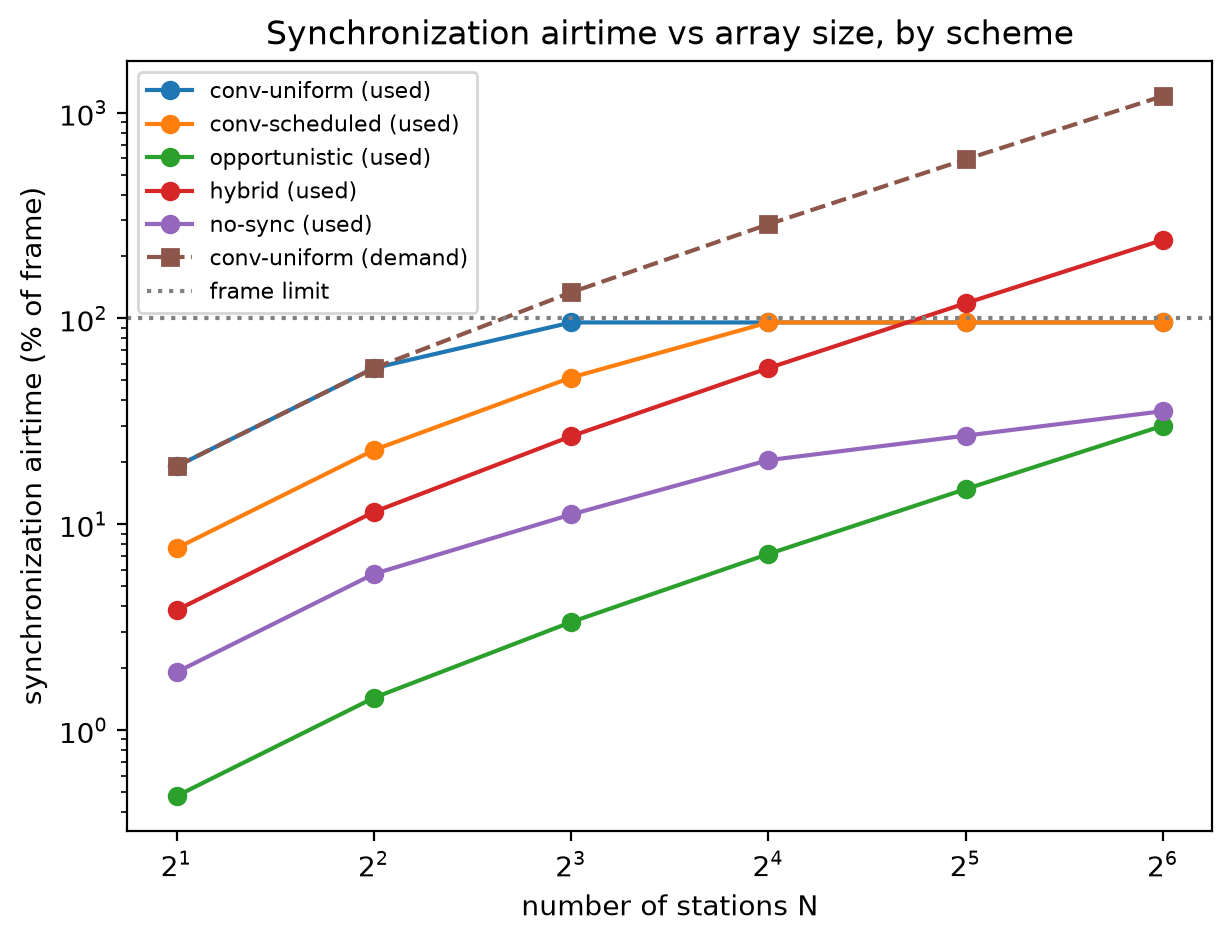
\includegraphics[width=\textwidth]{figures/figA2_airtime_vs_N.png}
      \begin{center}\scriptsize Synchronization airtime vs.\ array size, per scheme.\end{center}
    \end{column}
  \end{columns}
\end{frame}

% ---------------------------------------------------------------- 3
\begin{frame}{The conventional design rule --- and the claim of this work}
  \textbf{The field's rule:} synchronization rate is priced by
  \emph{oscillator quality}.
  \begin{itemize}
    \item Update-interval analyses derive re-synchronization cadence
          from oscillator and PLL phase noise (Mghabghab \& Nanzer,
          \emph{IEEE Access} 2021).
    \item BeamSync, AirSync, and the TDD-integrated calibration line
          all transmit \emph{synchronization-specific} signals ---
          references, preambles, or beamformed sync waveforms --- at a
          cadence set by clock drift.
  \end{itemize}
  \vspace{0.6em}
  \textbf{This work inverts the rule:}
  \begin{block}{}
    \centering
    When ordinary traffic carries the tracking, the required rate of
    dedicated two-way exchanges is set by the \emph{environment's}
    coherence time --- not by the clocks.
  \end{block}
\end{frame}

% ---------------------------------------------------------------- 4
\begin{frame}{The idea: ordinary transmissions as free phase observations}
  \begin{itemize}
    \item The array radiates data and sensing bursts constantly.
          Every time station $j$ overhears station $i$'s transmission,
          it observes a phase --- at \emph{zero marginal airtime}.
    \item Closest ancestor: Quitin \emph{et al.}\ (2013) extract
          frequency/phase from the modulated waveform of
          \emph{explicitly generated feedback packets}, referenced to
          a designated receiver's clock.
    \item Delta here: \textbf{no synchronization-specific transmission
          exists at all}. Arbitrary payload-bearing bursts between
          array elements are the observations, and the transmitting
          stations' own oscillators are steered in closed loop.
  \end{itemize}
  \vspace{0.4em}
  \begin{center}
    \small measured: phase extracted from unmodified random-data OFDM
    bursts is \emph{as good or better} than a dedicated preamble
    (4.78 vs.\ 8.75\,mrad per observation --- slide 12 explains why).
  \end{center}
\end{frame}

% ---------------------------------------------------------------- 5
\begin{frame}{The catch: an impossibility result}
  A one-way observation mixes two things that must not be confused:
  \[
    y_{ij} = \underbrace{\theta_i - \theta_j}_{\text{clock offset}}
           + \underbrace{\psi_{ij}}_{\text{propagation phase}} + n .
  \]
  Track the per-link state $x = [\theta,\ \omega,\ \psi]$
  (clock phase, clock frequency, path phase). One-way observations
  have measurement row $H_{\mathrm{free}} = [1,\ 0,\ 1]$: they see
  only the \emph{sum}.
  \begin{block}{Non-identifiability (proved)}
    The observability Gramian of $(F, H_{\mathrm{free}})$ has rank 2.
    Its null direction is exactly $(1, 0, -1)/\sqrt{2}$: \textbf{no
    amount of one-way data --- at any signal-to-noise ratio, over any
    duration --- can separate clock from path.}
  \end{block}
  Ablation confirms the stakes: a 2-state filter that ignores the path
  state steers the transmitter by the propagation phase ---
  $1327 \pm 100\mrad$, beam quality collapses to 62.6\%.
\end{frame}

% ---------------------------------------------------------------- 6
\begin{frame}{The fix: sparse dedicated two-way exchanges}
  \begin{itemize}
    \item A dedicated two-way exchange measures the clock offset
          \emph{alone}: the half-difference of the two directions
          cancels the (reciprocal) path,
          $\tfrac12\,\mathrm{wrap}(\varphi_{ij}-\varphi_{ji}) \to
          \theta_i-\theta_j$. Its measurement row $[1,\,0,\,0]$
          restores the Gramian to full rank.
    \item One such exchange every $K$ update intervals re-pins the
          clock/path decomposition; free observations track the clocks
          in between.
  \end{itemize}
  \begin{block}{The residual $\pi$ ambiguity, resolved with one bit}
    The half-difference observes $\mathrm{wrap}(2\theta)$ --- a 2-to-1
    map, so exactly two candidates $\{\hat\theta, \hat\theta+\pi\}$
    remain, and the wrong one is an attractor (zero innovation while
    the transmitters cancel). A periodic one-bit test,
    $\mathrm{sign}(\cos\theta_{\mathrm{err}})$, decides a two-element
    set: one bit is \emph{necessary and sufficient}. Measured under
    adverse acquisition (initial offset $2.2$\,rad): \textbf{12/12
    seeds lock anti-phase without the check, 0/12 with it}.
  \end{block}
\end{frame}

% ---------------------------------------------------------------- 7
\begin{frame}{When does the decomposition survive? A zero-fit boundary}
  \begin{columns}[T]
    \begin{column}{0.5\textwidth}
      Environment motion makes the path phase drift; the filter's
      gains misattribute the deterministic Doppler ramp to the
      clocks. The locked bias after $K$ intervals is
      $\approx \pi f_D T K$, giving the identifiability condition
      \[
        \boxed{\;\pi\, f_D\, T\, K \;<\; b\;}
      \]
      ($f_D$ Doppler frequency, $T$ update interval, $K$ exchange
      spacing, $b$ phase budget). \textbf{No oscillator parameter
      appears.}
      \begin{itemize}
        \item Predicted collapse: 0.066\,m/s ($K{=}10$),
              0.016\,m/s ($K{=}40$) at $b = 0.314$\,rad.
        \item Measured: within one grid step of both, no fitted
              constants; three regimes (free / biased / broken) with
              the predicted signatures.
      \end{itemize}
    \end{column}
    \begin{column}{0.48\textwidth}
      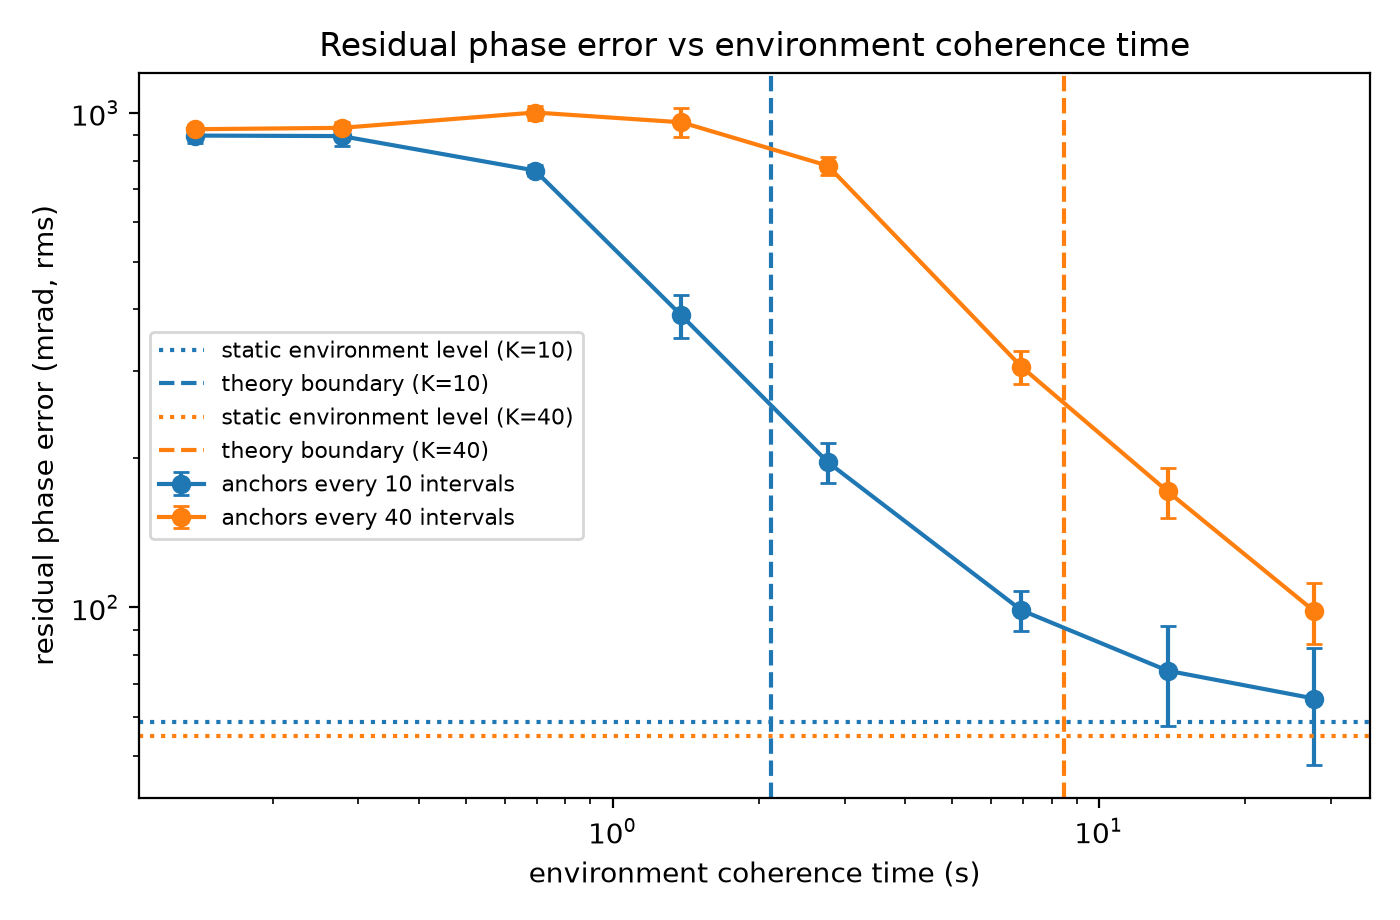
\includegraphics[width=\textwidth]{figures/expB_residual_vs_coherence_time.png}
      \begin{center}\scriptsize Residual vs.\ environment coherence time, two exchange cadences; dashed verticals = predicted boundaries.\end{center}
    \end{column}
  \end{columns}
\end{frame}

% ---------------------------------------------------------------- 8
\begin{frame}{Result 1: rarer dedicated exchanges \emph{improve} accuracy}
  \begin{columns}[T]
    \begin{column}{0.5\textwidth}
      Sweep the exchange spacing $K = 2 \to 320$ at $N=8$, static
      environment:
      \begin{itemize}
        \item $129.5\mrad$ at 66.9\% synchronization airtime
              $\;\longrightarrow\;$ $\mathbf{86.0 \pm 4.5\mrad}$ at
              \textbf{0.42\%}.
        \item Airtime cut $160\times$; the residual does not degrade
              --- it improves, because each two-way capture itself
              injects multipath measurement noise.
        \item Every point on the frontier beats the dedicated
              baseline ($193.3\mrad$ at 51.6\%) on \emph{both} axes.
      \end{itemize}
      \vspace{0.3em}
      \scriptsize Static-environment best case; sparsity is bounded
      by the slide-7 condition, not by clock drift.
    \end{column}
    \begin{column}{0.48\textwidth}
      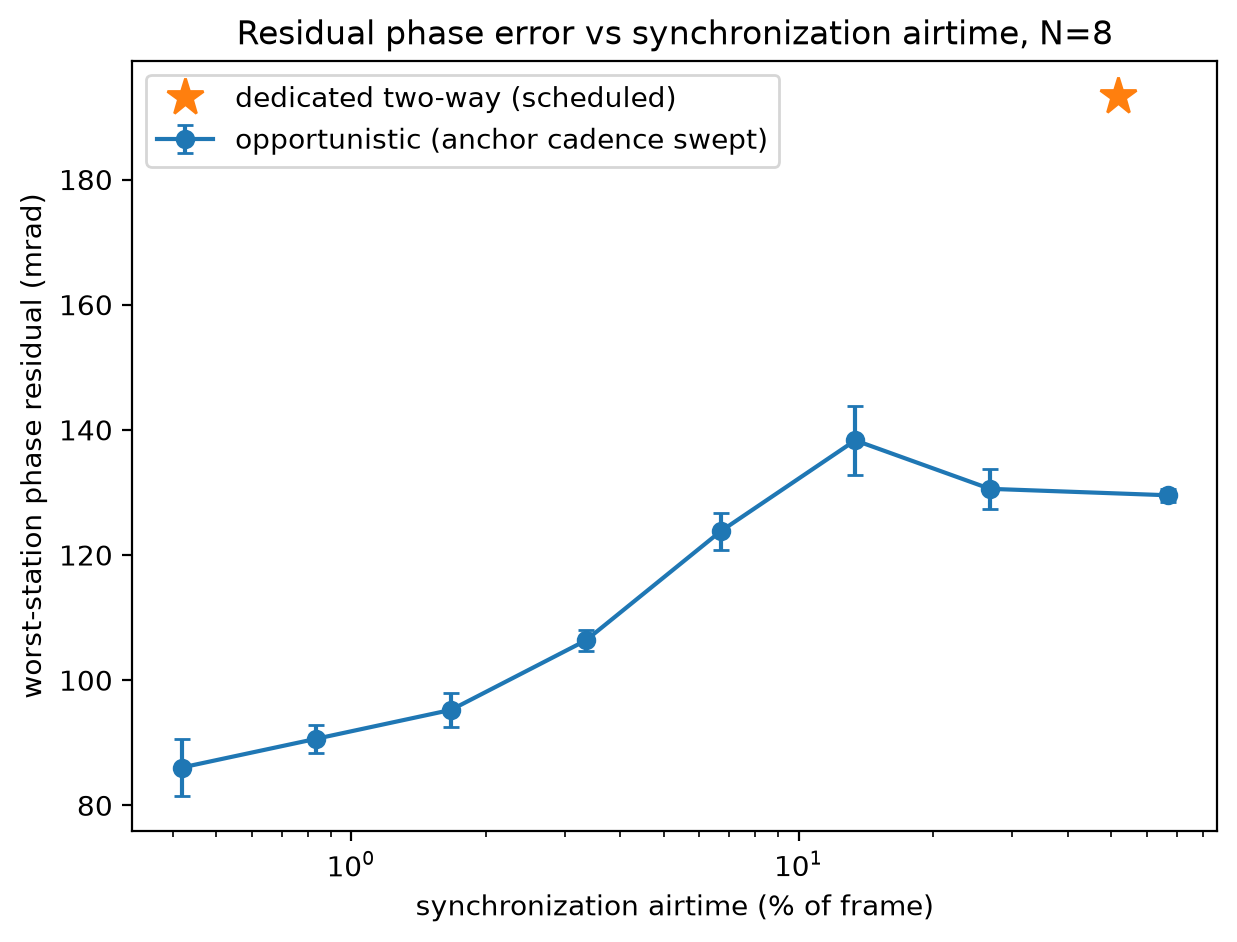
\includegraphics[width=\textwidth]{figures/figC1_exchange_frontier.png}
      \begin{center}\scriptsize Residual vs.\ dedicated-exchange airtime.\end{center}
    \end{column}
  \end{columns}
\end{frame}

% ---------------------------------------------------------------- 9
\begin{frame}{Result 2: free observations never hurt (hypothesis test)}
  \begin{columns}[T]
    \begin{column}{0.5\textwidth}
      An expert reviewer predicted a U-shaped error curve in a slowly
      varying environment: too many free observations should let
      channel motion masquerade as clock drift. Our theory predicted
      no U.
      \begin{itemize}
        \item 5 seeds, 4 environment speeds, observation rate
              $1\to20$ per interval, post-convergence statistics.
        \item Static: monotone improvement, $138.7 \to 41.7\mrad$.
        \item Moving: \emph{flat} --- the locked bias is independent
              of observation rate (290--327$\mrad$ over a $20\times$
              rate range at 0.02\,m/s).
      \end{itemize}
      \textbf{Verdict: no U-curve at any speed} --- the real tradeoff
      lives on the exchange-spacing axis (slide 7).
    \end{column}
    \begin{column}{0.48\textwidth}
      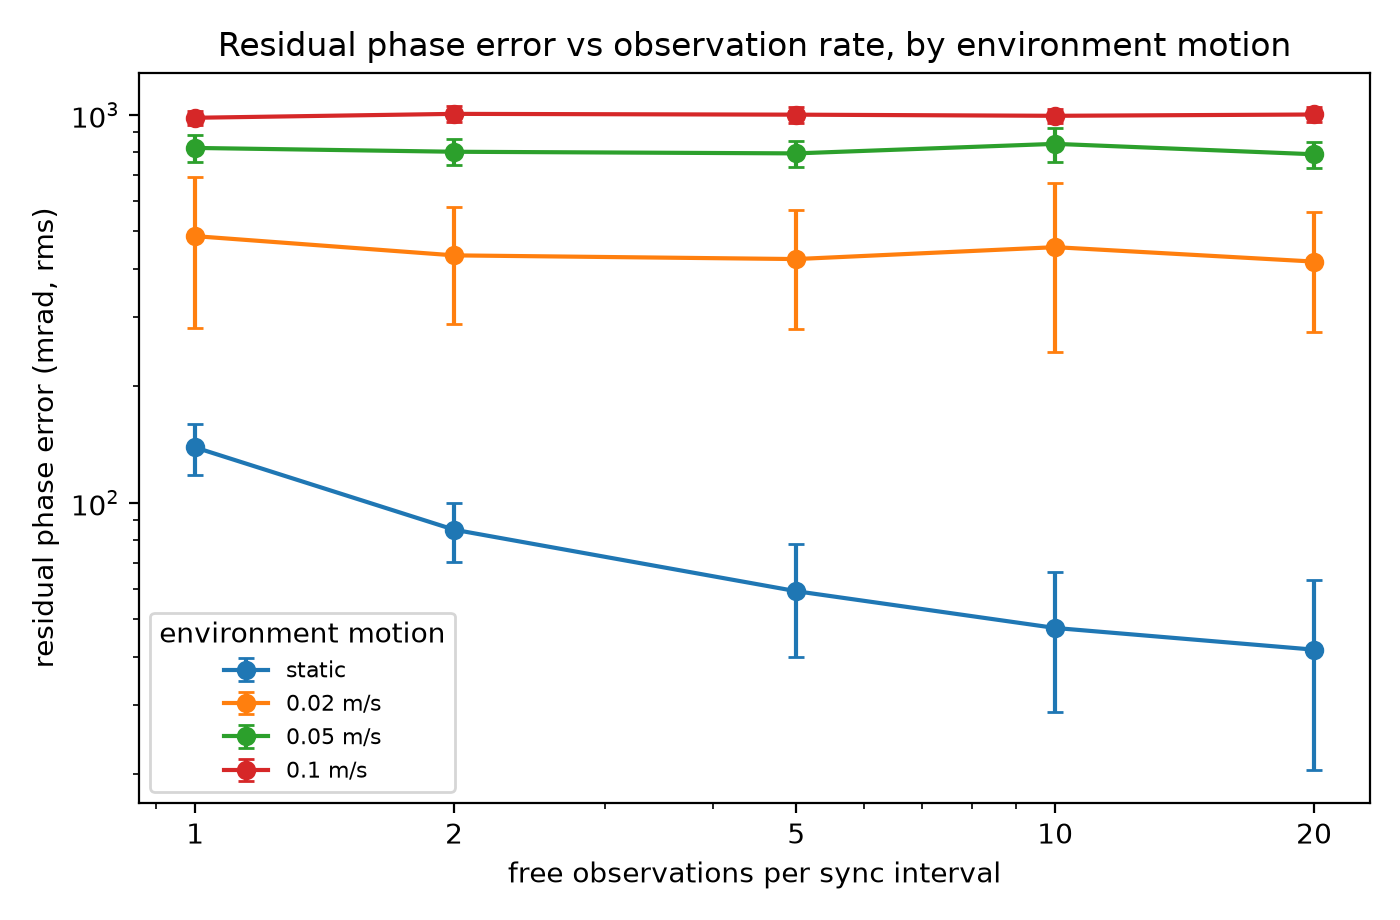
\includegraphics[width=\textwidth]{figures/expD_residual_vs_observation_rate.png}
      \begin{center}\scriptsize Residual vs.\ free-observation rate, per environment speed.\end{center}
    \end{column}
  \end{columns}
\end{frame}

% --------------------------------------------------------------- 10
\begin{frame}{Result 3: flat accuracy from 2 to 64 stations}
  \begin{columns}[T]
    \begin{column}{0.53\textwidth}
      \scriptsize
      \begin{tabular}{@{}lccc@{}}
        \toprule
        $N$ & opportunistic & conv.\ (scheduled) & conv.\ (uniform) \\
        \midrule
        2  & $55\mrad$ / 0.5\%  & $174\mrad$ / 7.6\%  & $113\mrad$ / 19.1\% \\
        8  & $106\mrad$ / 3.3\% & $193\mrad$ / 51.6\% & $2190\mrad$ / 95.6\% \\
        16 & $75\mrad$ / 7.2\%  & $443\mrad$ / 95.6\% & $2498\mrad$ / 95.6\% \\
        64 & $108\mrad$ / 30.1\% & $2072\mrad$ / 95.6\% & $2294\mrad$ / 95.6\% \\
        \bottomrule
      \end{tabular}
      \normalsize
      \begin{itemize}
        \item Opportunistic: $55\to108\mrad$ over a $32\times$ size
              change, beam quality $\geq 99.7\%$ throughout.
        \item A dense-exchange control ($K{=}5$) matches the accuracy
              but its exchange demand alone exceeds the frame at
              $N\geq32$: the saving comes from \emph{replacing}
              dedicated exchanges with free observations, not from
              the estimator.
      \end{itemize}
    \end{column}
    \begin{column}{0.48\textwidth}
      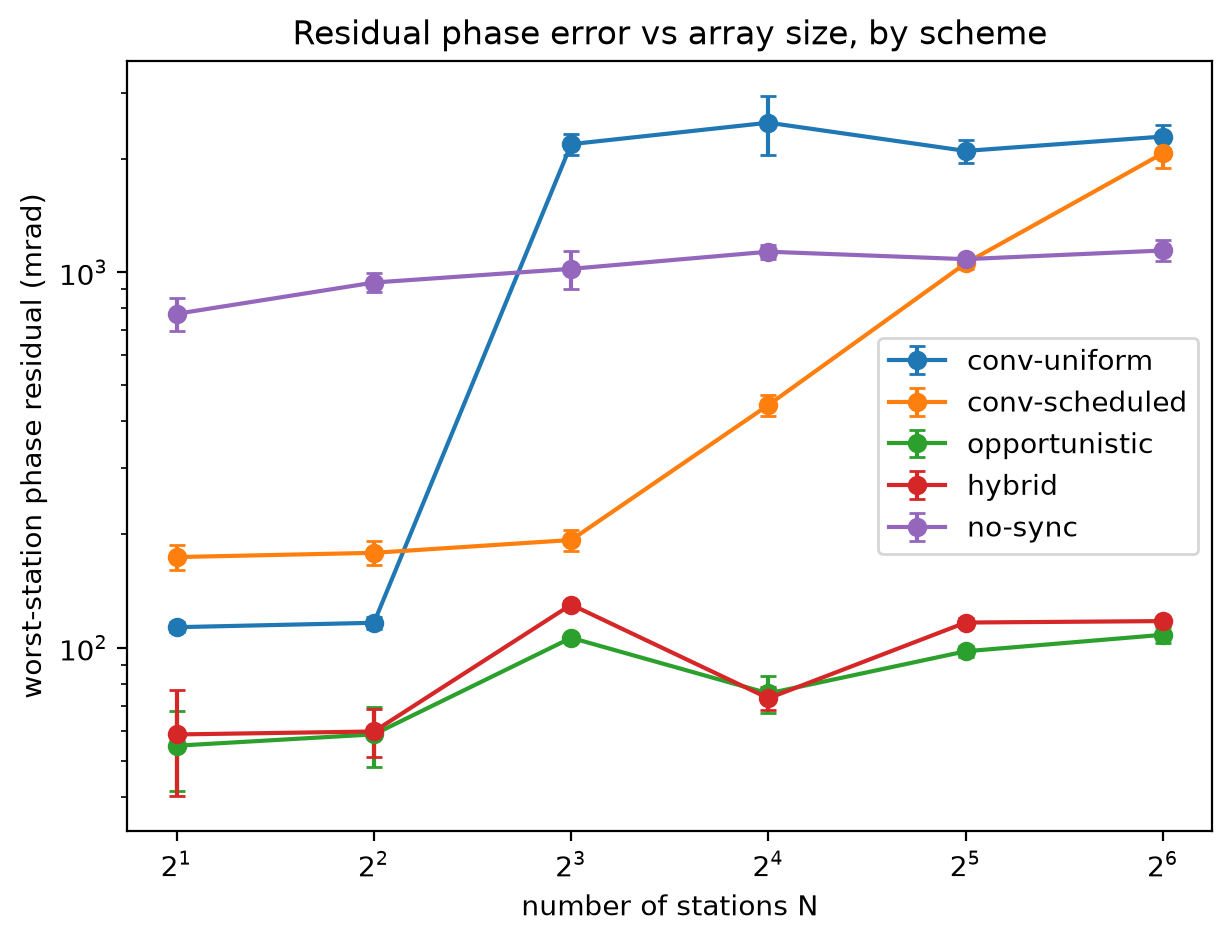
\includegraphics[width=\textwidth]{figures/figA1_residual_vs_N.png}
      \begin{center}\scriptsize Residual vs.\ array size, per scheme (log scale).\end{center}
    \end{column}
  \end{columns}
\end{frame}

% --------------------------------------------------------------- 11
\begin{frame}{Ablations: which components are load-bearing}
  \begin{columns}[T]
    \begin{column}{0.5\textwidth}
      \small
      \begin{tabular}{@{}lc@{}}
        \toprule
        configuration & residual \\
        \midrule
        full architecture & $54.7 \pm 13.2\mrad$ \\
        no path state (2-state filter) & $\mathbf{1327 \pm 100\mrad}$ \\
        no branch check (adverse acq.) & $\mathbf{3103 \pm 8\mrad}$ \\
        preamble instead of OFDM & $51.0 \pm 16.7\mrad$ \\
        no exchanges after acq.\ (static) & 40--62$\mrad$ \\
        \bottomrule
      \end{tabular}
      \normalsize
      \begin{itemize}
        \item Load-bearing: the clock/path decomposition and the
              branch check. Waveform: irrelevant at loop level.
        \item Static-environment surprise: realized decomposition
              drift runs $\sim$$1000\times$ below the worst-case
              bound --- a static channel never excites the
              unobservable direction. Dedicated exchanges then serve
              acquisition and branch resolution; under motion they
              are the only defense.
      \end{itemize}
    \end{column}
    \begin{column}{0.48\textwidth}
      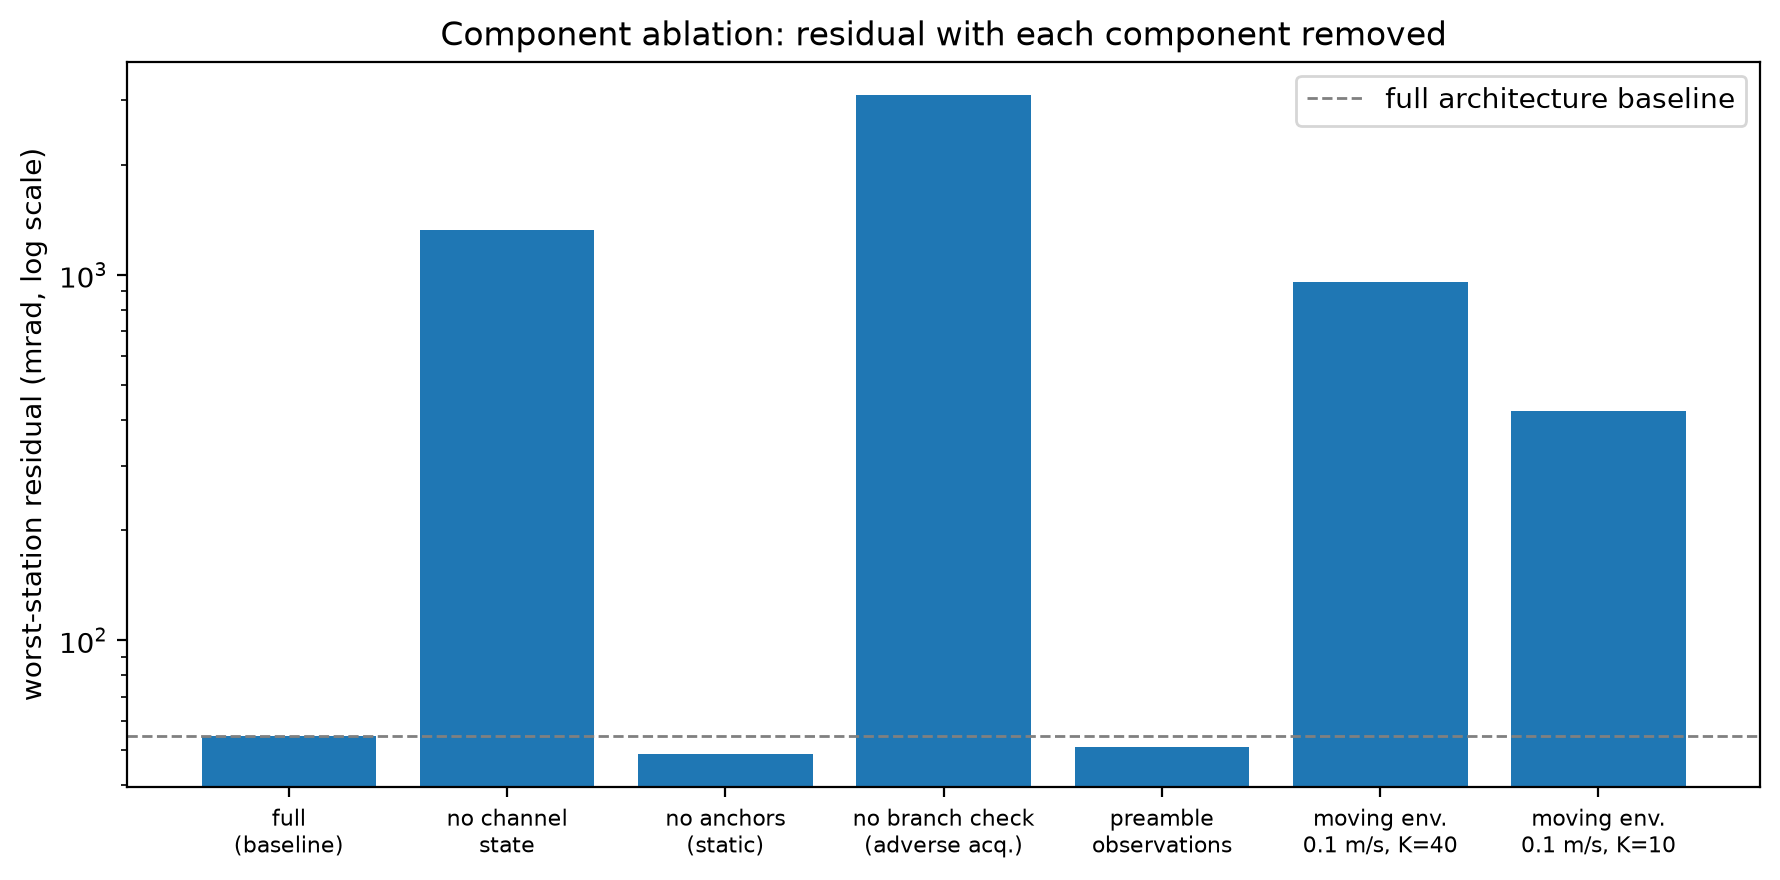
\includegraphics[width=\textwidth]{figures/fig_e1_ablation.png}
      \begin{center}\scriptsize Residual per ablated configuration.\end{center}
    \end{column}
  \end{columns}
\end{frame}

% --------------------------------------------------------------- 12
\begin{frame}{Why the data burst beats the dedicated preamble}
  \begin{columns}[T]
    \begin{column}{0.5\textwidth}
      \small
      Zero-fit model of per-observation error vs.\ capture length $L$:
      \[
        \sigma^2_{\mathrm{obs}}(L) \approx
        \underbrace{\tfrac{1/(2\,\mathrm{SNR}) + \sigma^2_{\mathrm{wpm}}}{L}}_{\text{thermal + white phase noise}}
        + \underbrace{\mathrm{walk}(L)}_{\substack{\text{intra-capture}\\ \text{oscillator random walk}}}
      \]
      \begin{itemize}
        \item The U-shape is real at every tested SNR; predictions
              track measurement within 10--25\% for $L \geq 511$.
        \item The 960-sample OFDM burst sits at the predicted
              optimum (4.25 predicted, 4.78$\mrad$ measured, 20\,dB);
              the stock preamble spans 4606 samples --- the
              walk-dominated branch (8.75$\mrad$).
        \item A length-optimized preamble closes most of the gap
              (5.83$\mrad$): \textbf{capture geometry, not waveform
              magic}.
      \end{itemize}
    \end{column}
    \begin{column}{0.48\textwidth}
      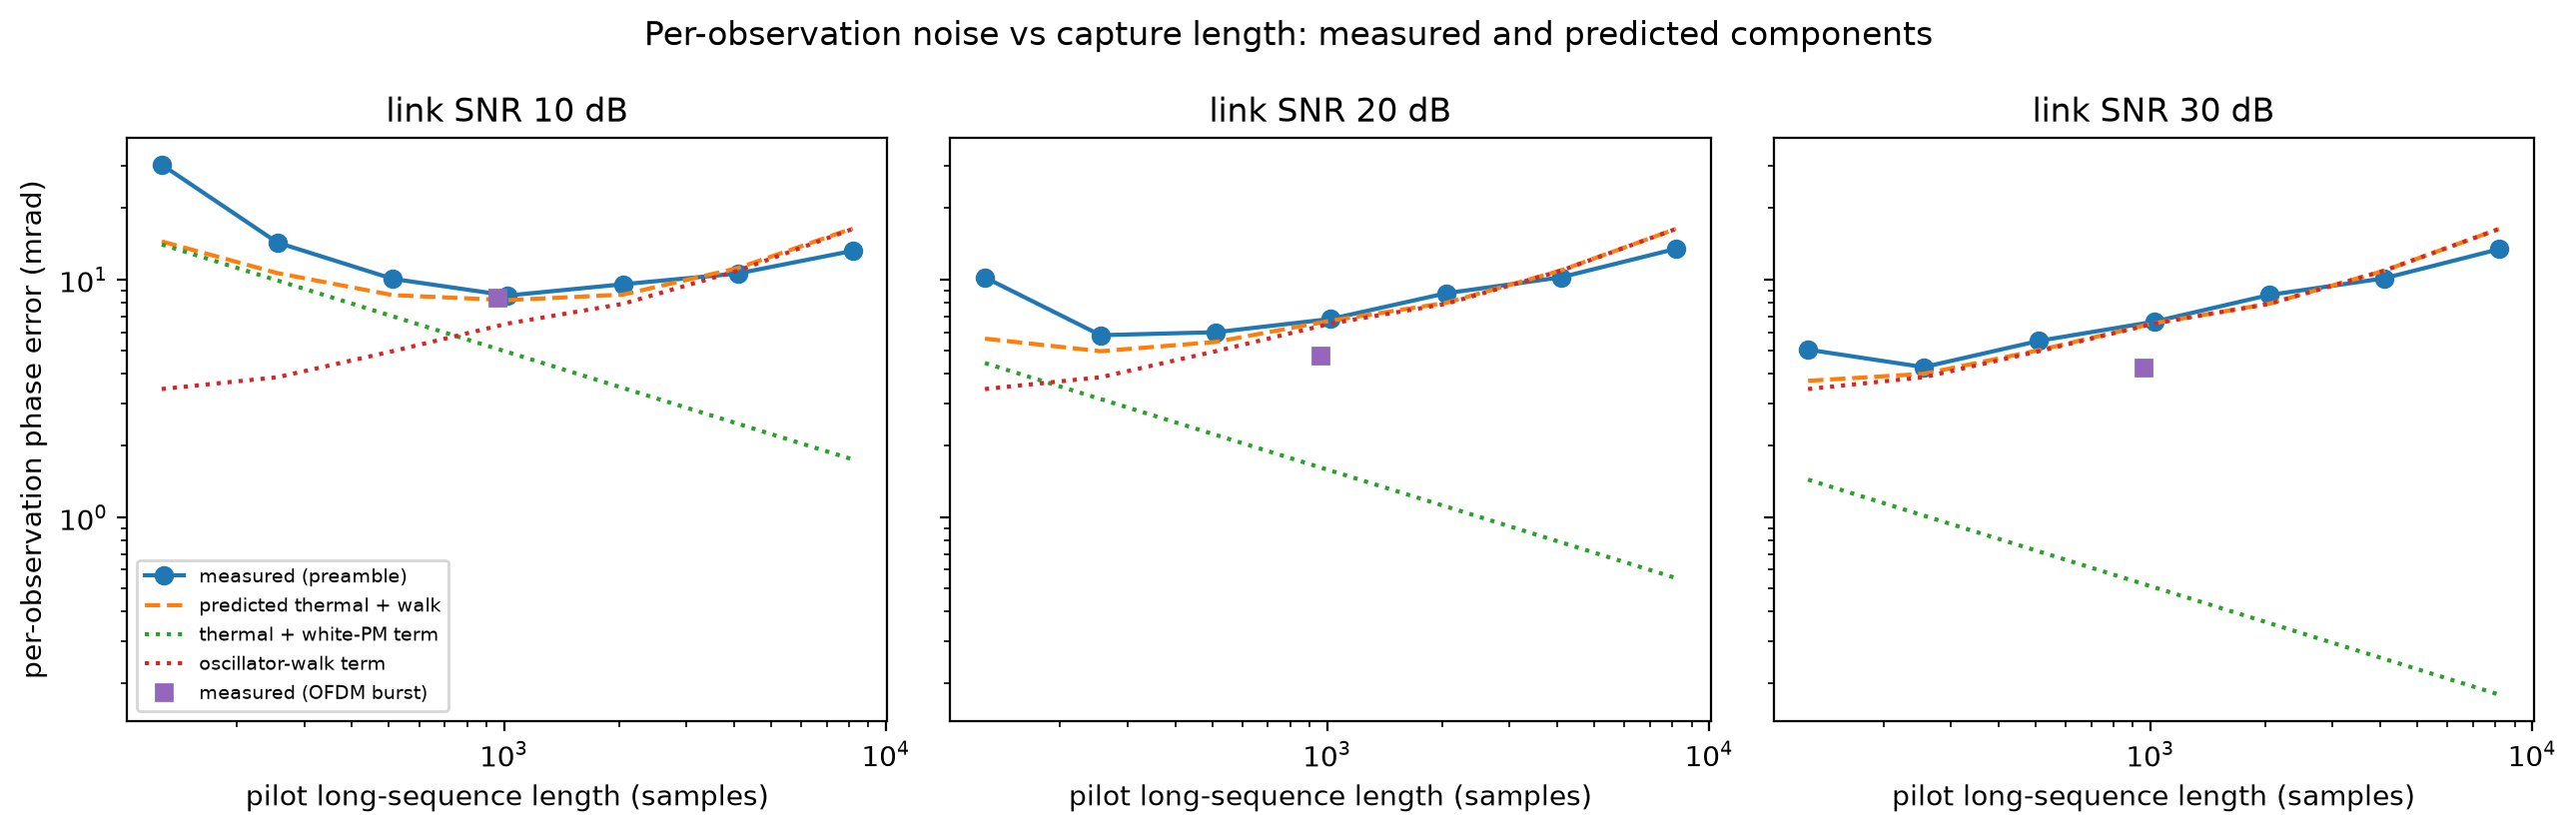
\includegraphics[width=\textwidth]{figures/fig_e2_capture_model.png}
      \begin{center}\scriptsize Per-observation error vs.\ capture length: measured points, predicted components (dashed).\end{center}
    \end{column}
  \end{columns}
\end{frame}

% --------------------------------------------------------------- 13
\begin{frame}{Limits, and where this sits in the literature}
  \textbf{Scope.} Simulation only: 915\,MHz, 1\,MHz bandwidth,
  multipath fading with ray-traced variants, path loss, timing
  jitter, four-term oscillator noise anchored to real datasheets, IQ
  imbalance, quantization, amplifier clipping, actuation latency.
  The frontier numbers are the static-environment best case; the
  slide-7 condition is the honest boundary.
  \vspace{0.5em}
  \small
  \begin{tabular}{@{}p{0.34\textwidth}p{0.60\textwidth}@{}}
    \toprule
    closest prior work & the gap \\
    \midrule
    Quitin \emph{et al.}\ 2013 & sync from \emph{explicitly generated}
    feedback packets, referenced to one receiver's clock; no
    clock/path separation problem arises \\
    Ngo \& Larsson (arXiv:2504.11411) & dedicated sync signal in
    engineered TDD overlap; inter-station channel \emph{assumed
    known}, so the ambiguity does not exist in their model \\
    Joint clock/channel estimation (Springer 2026) & dedicated
    pilots, receive-side; \emph{assumes} the separation is
    identifiable, with no conditions given \\
    Mghabghab \& Nanzer 2021 & re-sync interval priced by oscillator
    quality --- the design rule this work inverts \\
    \bottomrule
  \end{tabular}
\end{frame}

% --------------------------------------------------------------- 14
\begin{frame}{Takeaway}
  \begin{block}{}
    \centering\large
    Synchronization cadence is a property of the environment,\\
    not of the hardware.
  \end{block}
  \vspace{0.6em}
  \begin{enumerate}
    \item $\mathbf{86\mrad}$ residual at \textbf{0.42\%}
          synchronization airtime --- vs.\ $193\mrad$ at 52\% for
          dedicated two-way exchange --- and rarer exchanges
          \emph{improve} accuracy.
    \item Accuracy flat from \textbf{2 to 64 stations}
          ($55$--$108\mrad$, $\geq 99.7\%$ coherent gain) while every
          dedicated-signaling scheme tested is incoherent or
          frame-saturated at 64.
    \item The one thing that forces a dedicated exchange is
          environment motion, and the boundary is closed-form:
          $\pi f_D T K < b$ --- validated with zero fitted constants.
  \end{enumerate}
  \vspace{0.4em}
  \scriptsize All numbers: \texttt{phase\_sync\_idea/} experiment
  records (seeds 0--2; hypothesis test at 5 seeds). Simulation only;
  hardware validation is the natural next step.
\end{frame}

\end{document}
